\chapter{How tos}\label{chap:how_tos}


This is the best practice to reference stuff. For example, in order to refer to a definition, use \verb|\defref{def:positive_semidefinite}| (gives \defref{def:positive_semidefinite}) for each of the definitions. In this way, each reference is consistent. Similarly, the appropriate command shown in \tabref{tab:ref_commands}.



\section{How to reference stuff}\label{sec:general_definitions}


\begin{table}[h]
	\centering
	\begin{tabular}{|c|c|l|}
		\hline
		\texttt{\textbackslash secref\{YourLabel\}} & \secref{sec:general_definitions} &  \\ \hline
		\texttt{\textbackslash chapref\{YourLabel\}} & \chapref{chap:how_tos} &  \\ \hline
		\texttt{\textbackslash figref\{YourLabel\}} & \figref{fig:nyc_rn} &If using it with the label of a subfigure, \\&&includes the letter of subfigure as well.\\ \hline
		\texttt{\textbackslash equaref\{YourLabel\}} & \equaref{eq:equation_test} &  \\ \hline
		\texttt{\textbackslash problemref\{YourLabel\}} & \problemref{prob:example} &  \\ \hline
		\texttt{\textbackslash defref\{YourLabel\}} & \defref{def:positive_semidefinite} &  \\ \hline
		\texttt{\textbackslash exref\{YourLabel\}} & \exref{ex:example} &  \\ \hline
		\texttt{\textbackslash tabref\{YourLabel\}} &  \tabref{tab:ref_commands} & Chooses a specific figure, \\&&use only when it's clear to which \\&&figure you are talking about \\ \hline
		\texttt{\textbackslash subfigref\{YourLabel\}} & \subfigref{fig:nyc_simplified_roads} &  \\ \hline
		\texttt{\textbackslash appref\{YourLabel\}} & Appendix &  \\ \hline
	\end{tabular}
	\caption{Proposed reference commands}\label{tab:ref_commands}
\end{table}



\begin{problem}\label{prob:example} 
	Given a transportation network $\mathcal{G}$ and a set of vehicles $\mathcal{A}$, solve:
	\begin{align}
		\text{min}& 
		\mathcal{J}_T = \sum_{a \in \mathcal{A}} \sum_{(u, v) \in \mathcal{E}} T^a_{ u,v} V^a_{u,v}
		\nonumber\\
		\text{s.t.} &\nonumber\\
		&\sum_{u \in \mathcal{V}} V^a_{u, v} - \sum_{w \in \mathcal{V}} V^a_{v, w} = 0 \quad \forall a \in \mathcal{A}, v \in \mathcal{V} \setminus \{\underline{s_a}, \bar{t_a}\} \label{eq:flow_conservation_graph_u} \\
		&\sum_{ u \in \mathcal{N}^+_{\underline{s_a}} }V^a_{ \underline{s_a},u} = 1 \quad \forall a \in \mathcal{A} \label{eq:flow_cons_arrival_graph_u}\\
		&\sum_{u \in \mathcal{N}^-_{\bar{t_a}} } V^a_{u, \bar{t_a}} = 1 \quad \forall a \in \mathcal{A} \label{eq:flow_cons_departure_graph_u}\\
		\nonumber
	\end{align}
\end{problem}

\begin{definition}\label{def:positive_semidefinite}
	A symmetric matrix $A$ is said to be positive semidefinite if, for any non-zero column vector $x$, the following inequality holds:
	\begin{equation}
		x^T Ax \geq 0\label{eq:equation_test}
	\end{equation}
	Here, $x^T$ represents the transpose of the vector $x$, and $x^T Ax$ is the quadratic form associated with the matrix $A$. Another way to express positive semidefiniteness is in terms of eigenvalues. A symmetric matrix $A$ is positive semidefinite if and only if all of its eigenvalues are non-negative.\\
	Mathematically, $A \succeq 0 $ indicates positive semidefiniteness.
\end{definition}

\begin{example}\label{ex:example}
	This is an example
\end{example}


\begin{figure}[tbh]
	\centering
	\begin{subfigure}[b]{0.32\textwidth}
		\centering
		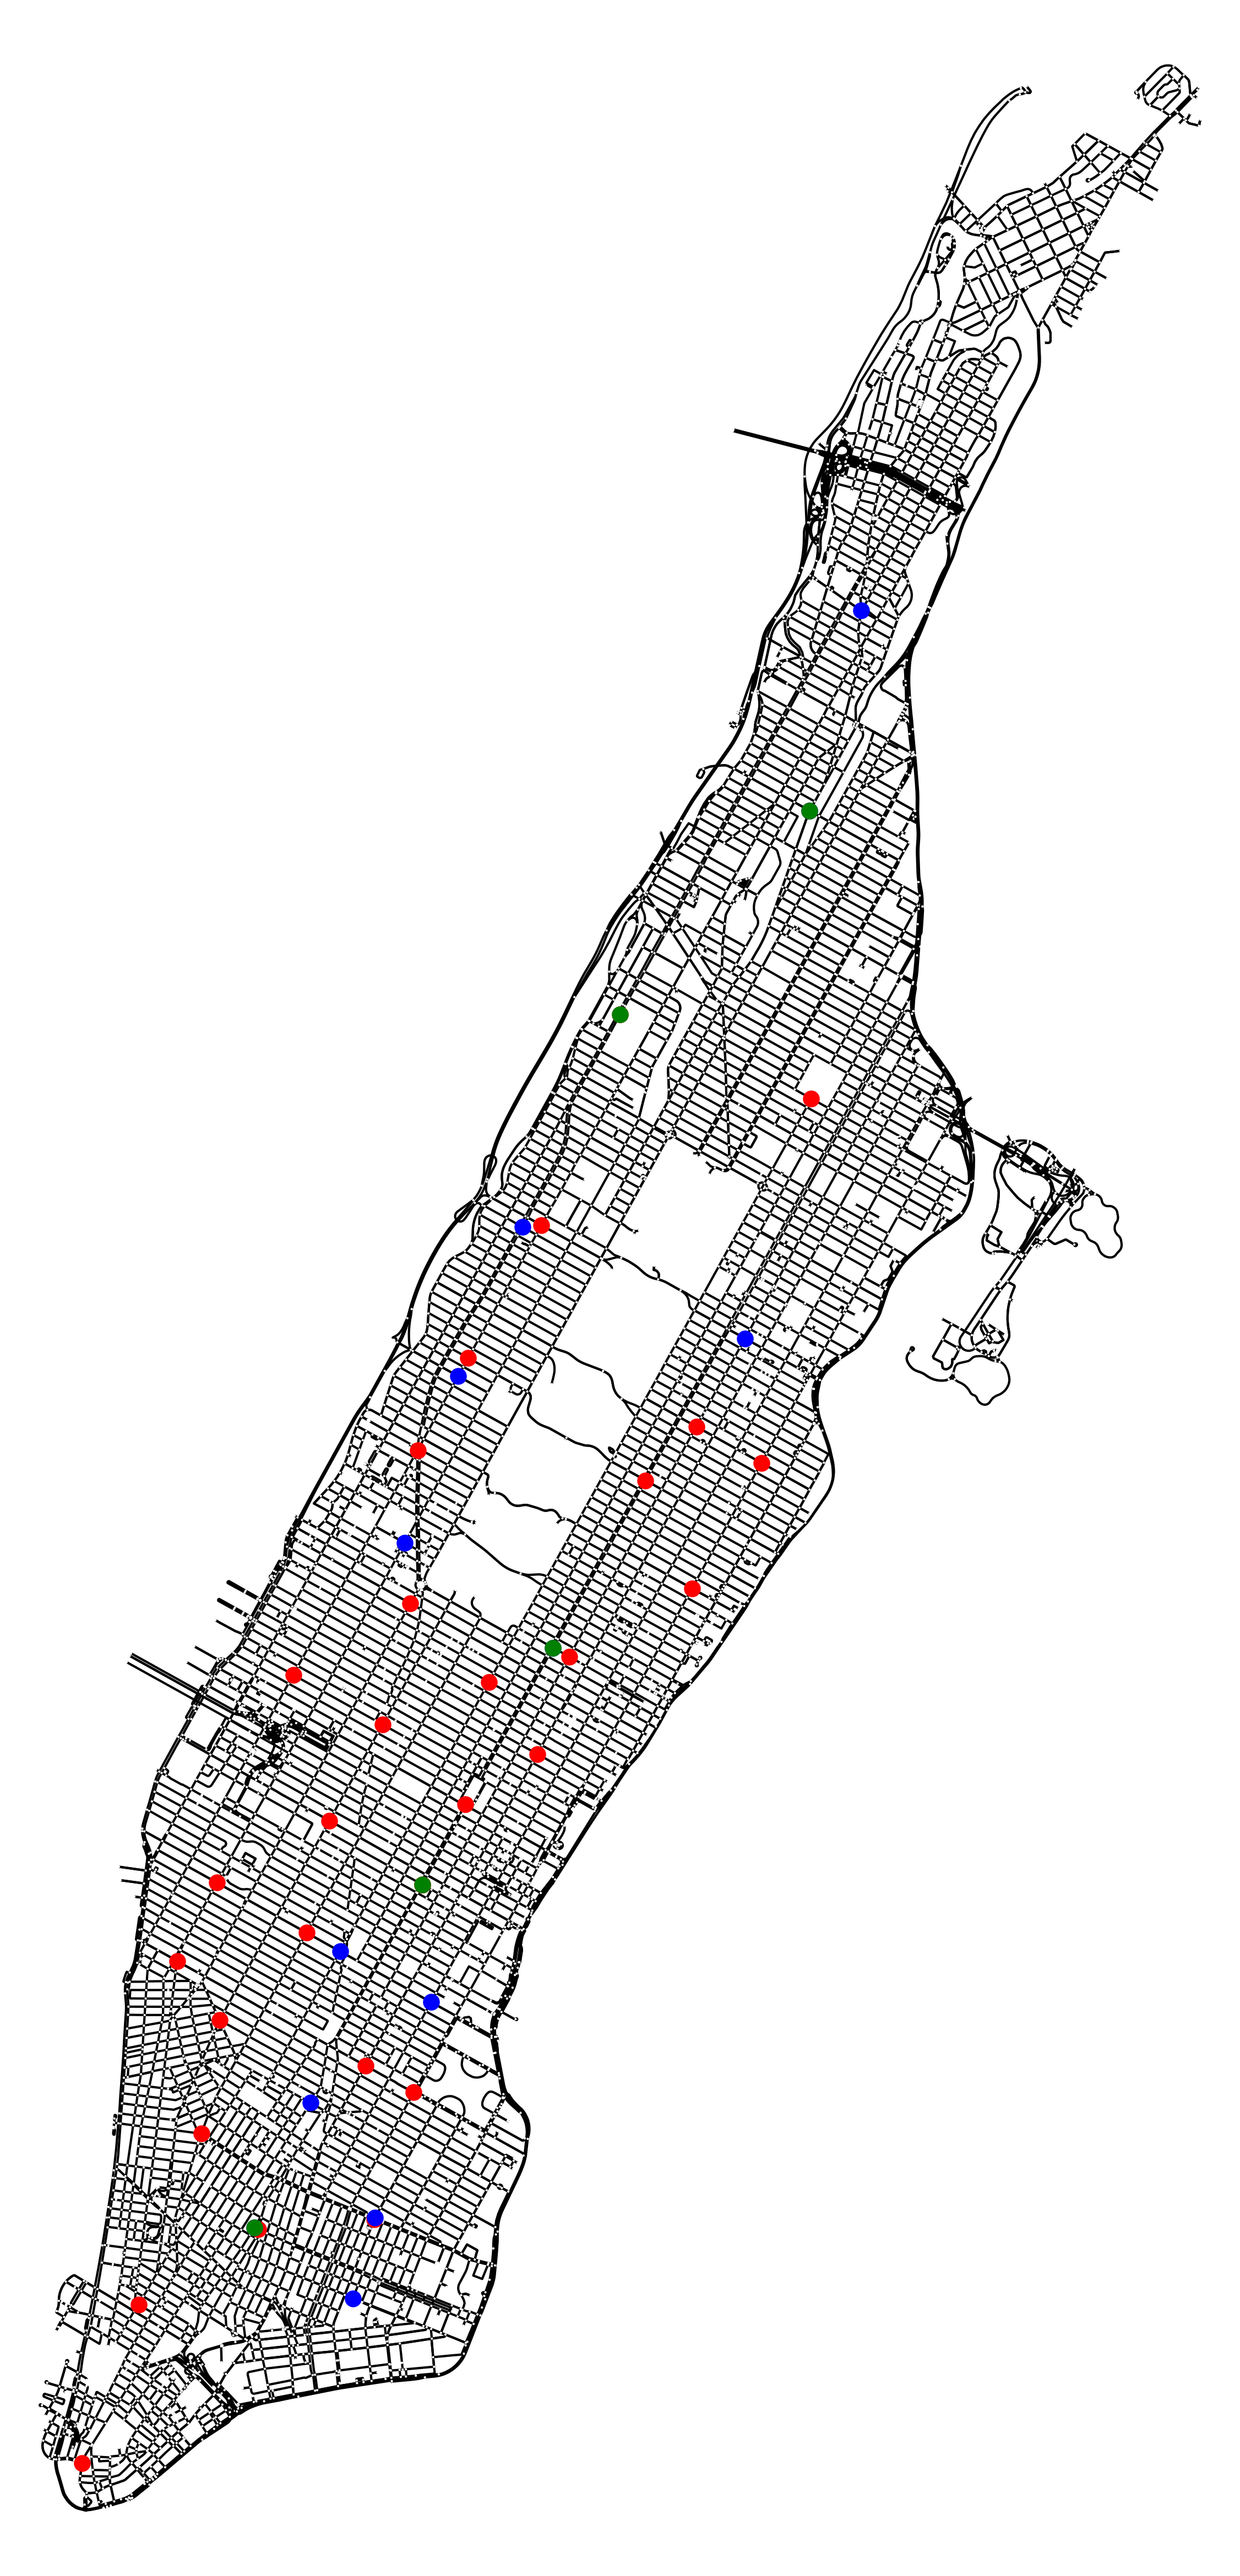
\includegraphics[width=\textwidth]{assets/img/new_york_vanilla_info.png}
		\caption{}
		\label{fig:nyc_rn_info}
	\end{subfigure}
	\begin{subfigure}[b]{0.32\textwidth}
		\centering
		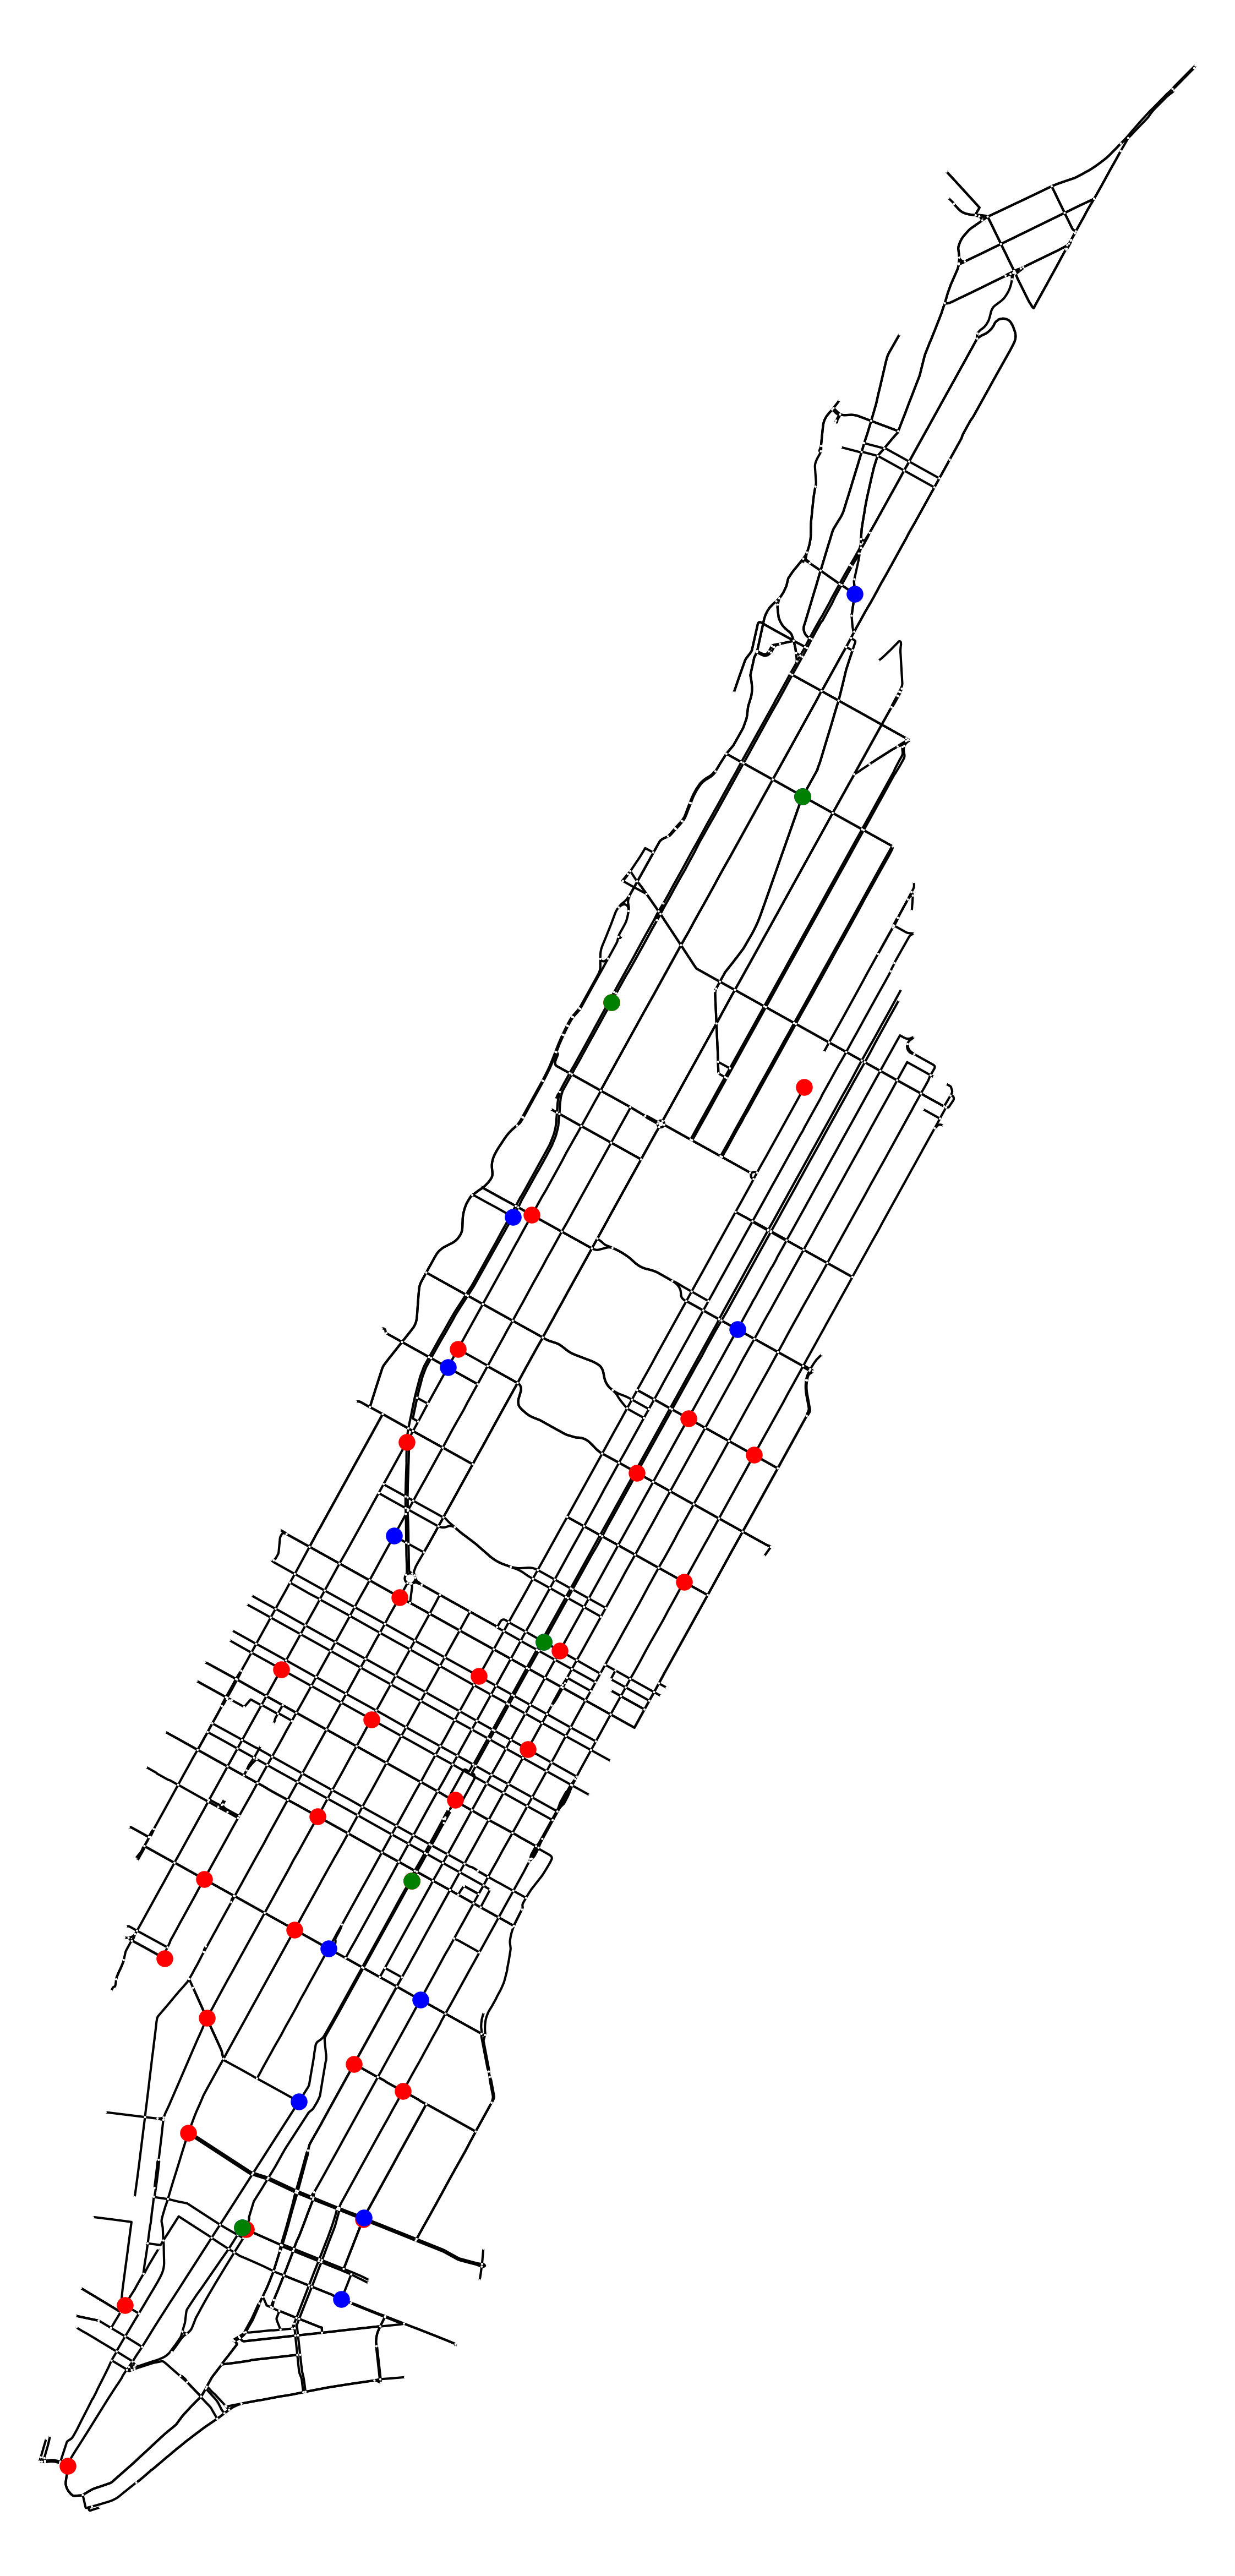
\includegraphics[width=\textwidth]{assets/img/new_york_simplified_info.png}
		\caption{}
		\label{fig:nyc_simplified_info}
	\end{subfigure}
	\begin{subfigure}[b]{0.32\textwidth}
		\centering
		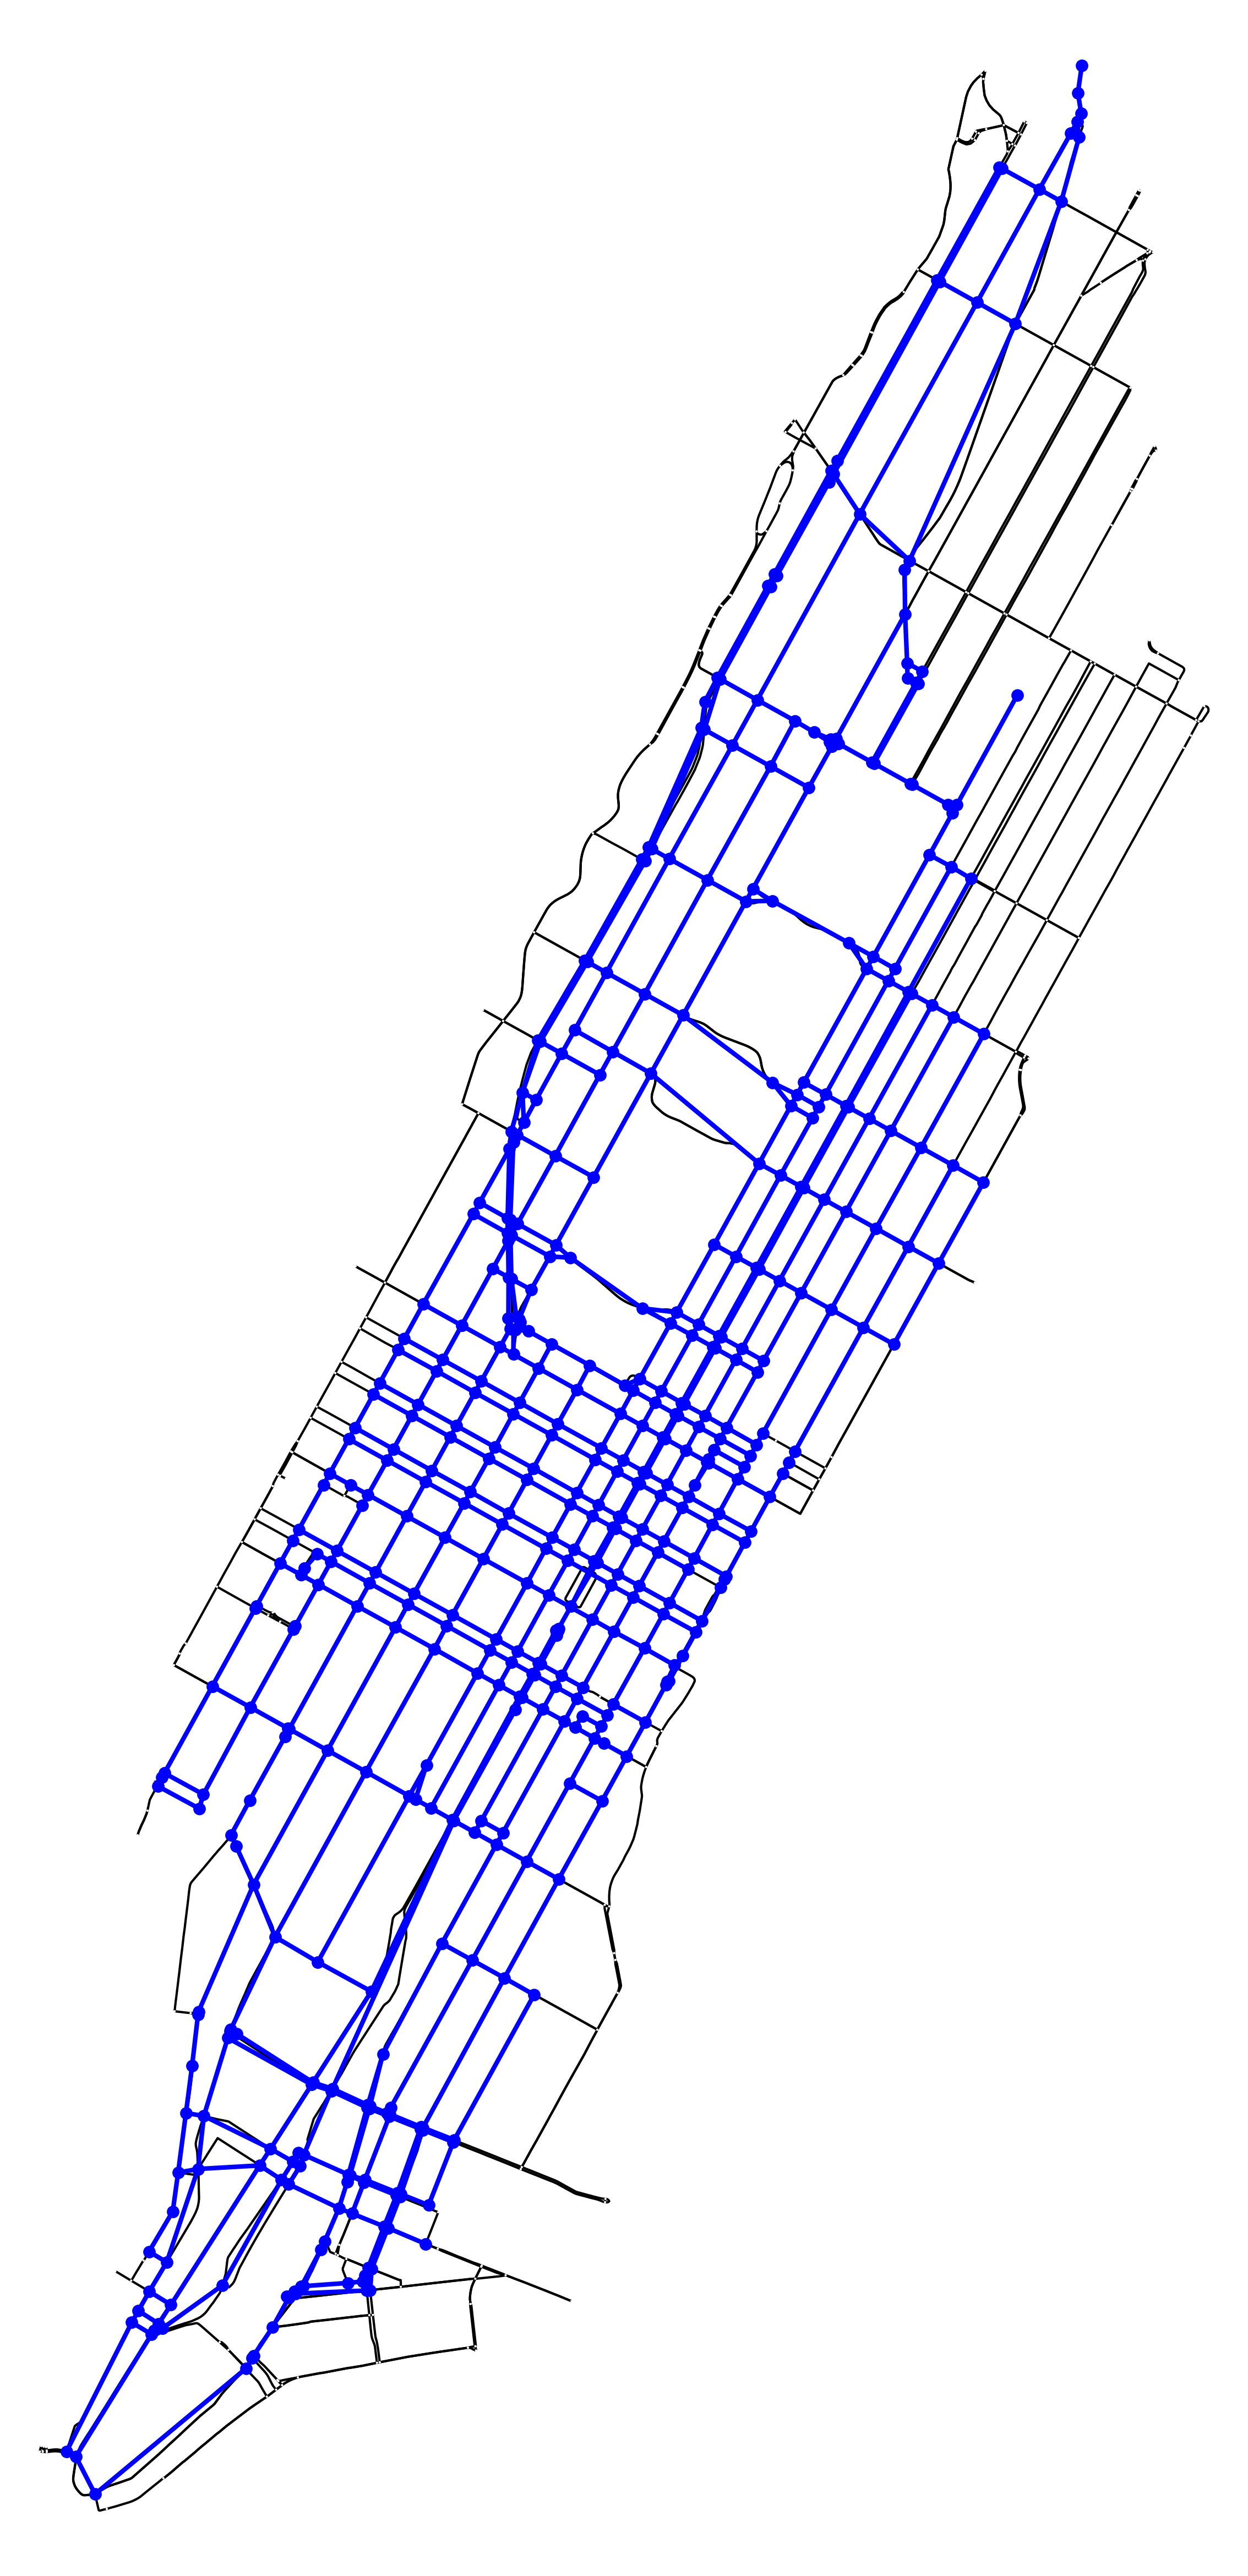
\includegraphics[width=\textwidth]{assets/img/new_york_simplified_roads.png}
		\caption{}
		\label{fig:nyc_simplified_roads}
	\end{subfigure}
	
	\caption[Title In the TOC]{Description }
	\label{fig:nyc_rn}
\end{figure}











